\documentclass[12pt,a4paper]{article}

\usepackage[in, plain]{fullpage}
\usepackage{array}
\usepackage{../../../pas-math}
\usepackage{../../../moncours}


%\usepackage{pas-cours}
%-------------------------------------------------------------------------------
%          -Packages nécessaires pour écrire en Français et en UTF8-
%-------------------------------------------------------------------------------
\usepackage[utf8]{inputenc}
\usepackage[frenchb]{babel}
\usepackage[T1]{fontenc}
\usepackage{lmodern}
\usepackage{textcomp}



%-------------------------------------------------------------------------------

%-------------------------------------------------------------------------------
%                          -Outils de mise en forme-
%-------------------------------------------------------------------------------
\usepackage{hyperref}
\hypersetup{pdfstartview=XYZ}
%\usepackage{enumerate}
\usepackage{graphicx}
\usepackage{multicol}
\usepackage{tabularx}
\usepackage{multirow}


\usepackage{anysize} %%pour pouvoir mettre les marges qu'on veut
%\marginsize{2.5cm}{2.5cm}{2.5cm}{2.5cm}

\usepackage{indentfirst} %%pour que les premier paragraphes soient aussi indentés
\usepackage{verbatim}
\usepackage{enumitem}
\usepackage[usenames,dvipsnames,svgnames,table]{xcolor}

\usepackage{variations}

%-------------------------------------------------------------------------------


%-------------------------------------------------------------------------------
%                  -Nécessaires pour écrire des mathématiques-
%-------------------------------------------------------------------------------
\usepackage{amsfonts}
\usepackage{amssymb}
\usepackage{amsmath}
\usepackage{amsthm}
\usepackage{tikz}
\usepackage{xlop}
%-------------------------------------------------------------------------------



%-------------------------------------------------------------------------------


%-------------------------------------------------------------------------------
%                    - Mise en forme avancée
%-------------------------------------------------------------------------------

\usepackage{ifthen}
\usepackage{ifmtarg}


\newcommand{\ifTrue}[2]{\ifthenelse{\equal{#1}{true}}{#2}{$\qquad \qquad$}}

%-------------------------------------------------------------------------------

%-------------------------------------------------------------------------------
%                     -Mise en forme d'exercices-
%-------------------------------------------------------------------------------
%\newtheoremstyle{exostyle}
%{\topsep}% espace avant
%{\topsep}% espace apres
%{}% Police utilisee par le style de thm
%{}% Indentation (vide = aucune, \parindent = indentation paragraphe)
%{\bfseries}% Police du titre de thm
%{.}% Signe de ponctuation apres le titre du thm
%{ }% Espace apres le titre du thm (\newline = linebreak)
%{\thmname{#1}\thmnumber{ #2}\thmnote{. \normalfont{\textit{#3}}}}% composants du titre du thm : \thmname = nom du thm, \thmnumber = numéro du thm, \thmnote = sous-titre du thm

%\theoremstyle{exostyle}
%\newtheorem{exercice}{Exercice}
%
%\newenvironment{questions}{
%\begin{enumerate}[\hspace{12pt}\bfseries\itshape a.]}{\end{enumerate}
%} %mettre un 1 à la place du a si on veut des numéros au lieu de lettres pour les questions 
%-------------------------------------------------------------------------------

%-------------------------------------------------------------------------------
%                    - Mise en forme de tableaux -
%-------------------------------------------------------------------------------

\renewcommand{\arraystretch}{1.7}

\setlength{\tabcolsep}{1.2cm}

%-------------------------------------------------------------------------------



%-------------------------------------------------------------------------------
%                    - Racourcis d'écriture -
%-------------------------------------------------------------------------------

% Angles orientés (couples de vecteurs)
\newcommand{\aopp}[2]{(\vec{#1}, \vec{#2})} %Les deuc vecteurs sont positifs
\newcommand{\aopn}[2]{(\vec{#1}, -\vec{#2})} %Le second vecteur est négatif
\newcommand{\aonp}[2]{(-\vec{#1}, \vec{#2})} %Le premier vecteur est négatif
\newcommand{\aonn}[2]{(-\vec{#1}, -\vec{#2})} %Les deux vecteurs sont négatifs

%Ensembles mathématiques
\newcommand{\naturels}{\mathbb{N}} %Nombres naturels
\newcommand{\relatifs}{\mathbb{Z}} %Nombres relatifs
\newcommand{\rationnels}{\mathbb{Q}} %Nombres rationnels
\newcommand{\reels}{\mathbb{R}} %Nombres réels
\newcommand{\complexes}{\mathbb{C}} %Nombres complexes


%Intégration des parenthèses aux cosinus
\newcommand{\cosP}[1]{\cos\left(#1\right)}
\newcommand{\sinP}[1]{\sin\left(#1\right)}


%Probas stats
\newcommand{\stat}{statistique}
\newcommand{\stats}{statistiques}
%-------------------------------------------------------------------------------

%-------------------------------------------------------------------------------
%                    - Mise en page -
%-------------------------------------------------------------------------------

\newcommand{\twoCol}[1]{\begin{multicols}{2}#1\end{multicols}}


\setenumerate[1]{font=\bfseries,label=\textit{\alph*})}
\setenumerate[2]{font=\bfseries,label=\arabic*)}


%-------------------------------------------------------------------------------
%                    - Elements cours -
%-------------------------------------------------------------------------------





%\makeatletter
%\renewcommand*{\@seccntformat}[1]{\csname the#1\endcsname\hspace{0.1cm}}
%\makeatother


%\author{Olivier FINOT}
\date{}
\title{}

\graphicspath{{./img/}}

\lhead{Seq 3: Fractions}
\rhead{O. FINOT}
%
%\rfoot{Page \thepage}
\begin{document}
%\maketitle




\chap[num=5, color=red]{Nombres relatifs}{\today }

\begin{myobj}
	\begin{itemize}
		
		\item Construire le symétrique d’un point ou d'une figure par rapport à une droite à la main où à l’aide d’un logiciel;
		\item Construire le symétrique d’un point ou d'une figure par rapport à un point, à la main où à l’aide d’un logiciel;
		\item Utiliser les propriétés de la symétrie axiale ou centrale;
		\item Identifier des symétries dans des figures.		
	\end{itemize}
\end{myobj}

\begin{mycomp}
	\begin{itemize}
		\item \kw{Chercher (Ch2)} :  s’engager    dans    une    démarche    scientifique, observer, questionner, manipuler, expérimenter (sur une feuille de papier, avec des objets, à l’aide de logiciels), émettre des hypothèses, chercher des exemples ou des contre-exemples, simplifier ou particulariser une situation, émettre une conjecture ;
		\item \kw{Raisonner (Ra3)} :  démontrer : utiliser un raisonnement logique et des règles établies (propriétés, théorèmes, formules) pour parvenir à une conclusion ;
		\item \kw{Communiquer (Co2)} :  expliquer à l’oral ou à l’écrit (sa démarche, son raisonnement, un calcul, un protocole   de   construction   géométrique, un algorithme), comprendre les explications d’un autre et argumenter dans l’échange ; 
		
	\end{itemize}
\end{mycomp}




\section{Définitions}

\begin{mydef}
	$a$ et $b$ sont deux nombres ($b$ $\neq$ 0). Le \hspace{3cm} de $a$ par $b$ se note $a \div b$ ou $\dfrac{a}{b}$, en \hspace{5cm}.
\end{mydef}

\begin{myex}
	%\begin{itemize}
		%\item 
		Le quotient de 5 par 4 est $\dfrac{5}{4}$, c'est le nombre qui multiplié par 4 donne 5. 
		\begin{equation*}
			\dfrac{5}{4} \times 4 = 
		\end{equation*}

		%\item Le quotient de 2 par 3 est $\dfrac{2}{3}$, c'est le nombre qui multiplié par 3 donne 2. $\dfrac{2}{3} \times 3 = 2 $.
	%\end{itemize}
\end{myex}

\begin{mydef}
	Si $a$ et $b$ sont entiers, alors $\dfrac{a}{b}$ est une \hspace{3cm}. $a$ est le \hspace*{3cm} et $b$ est le \hspace*{3cm}.	
	
\end{mydef}

\begin{center}
	\includegraphics*[scale=0.5]{def_2}
\end{center}

\begin{myex}
	$\dfrac{\num{4.2}}{\num{2}}$, $\dfrac{\num{5}}{\num{2.4}}$, $\dfrac{\num{1.3}}{\num{3.7}}$ et $\dfrac{\num{2}}{\num{3}}$ sont toutes des écritures fractionnaires, mais seule \hspace{2cm} est une fraction.
\end{myex}

\newpage

\section{Des nombres pour se repérer et à comparer}

\subsection{Repérage}

\begin{mydef}
	Sur une droite graduée, chaque point est repéré par un nombre relatif, son %\kw{abscisse}.
\end{mydef}


\begin{myex}
	\begin{center}
		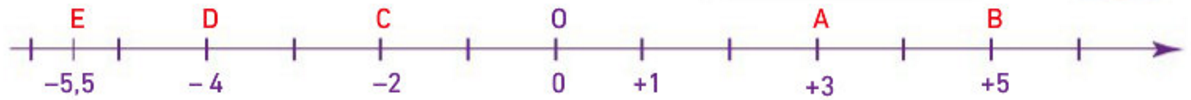
\includegraphics[scale=0.5]{img/droite2}		
	\end{center}

	\begin{multicols}{2}
		\begin{itemize}
		\item L'abscisse du point A est %+3;
		\item L'abscisse du point B est %+5;
		\item L'abscisse du point C est %-2;
		\item L'abscisse du point D est %-4.
		\item L'abscisse du point E est %\num{-5.5};
		\item L'abscisse du point O est %0;
	\end{itemize}
	\end{multicols}
\end{myex}


\begin{mydefs}
	\begin{itemize}
		\item Un repère orthogonal est formé par deux droites graduées perpendiculaires et de même origine. La droite horizontale est l'\hspace{6cm}, la verticale est l'%\kw{axe des ordonnées}.
		
		\item Un point du plan est repéré par deux nombres relatifs, ses %\kw{coordonnées}. 
		
		Le premier nombre est son \hspace{4cm}, le second son \hspace{4cm}. On note ces coordonnées $(abscisse \: ; \: ordonnée)$.
	\end{itemize}
\end{mydefs}


\begin{myexs}
	
		\begin{center}
			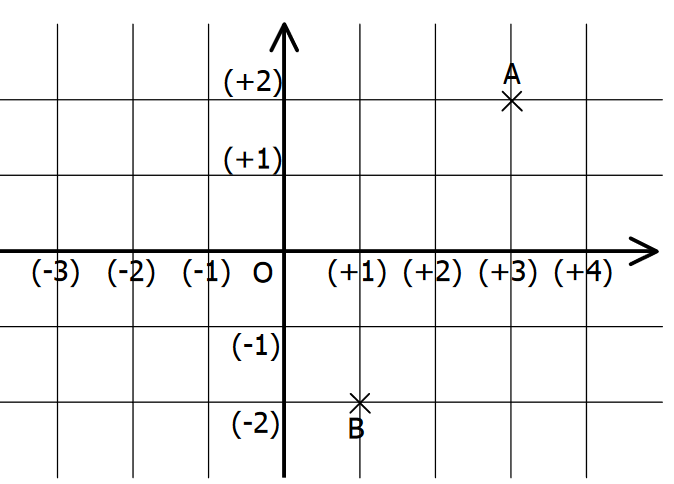
\includegraphics[scale=0.4]{repere}
		\end{center}
	

	\begin{itemize}
		\item L'abscisse du point $A$ est +3, son ordonnée est +2, ses coordonnées sont $(+3; +2)$.
		
		\item L'abscisse du point $B$ est +1, son ordonnée est -2, ses coordonnées sont $(+1; -2)$.
	\end{itemize}

\end{myexs}


\subsection{Comparaison}

\end{document}

